\documentclass{ctexart}

\usepackage{graphicx}
\usepackage{setspace}
\usepackage{booktabs}
\usepackage{amsmath} 
\usepackage{enumitem}
\usepackage{geometry}
\geometry{margin=2.5cm}

\numberwithin{figure}{section}
\renewcommand{\thefigure}{\thesection-\arabic{figure}}
\numberwithin{equation}{section}
\renewcommand{\theequation}{\thesection-\arabic{equation}}
\numberwithin{table}{section}
\renewcommand{\thetable}{\thesection-\arabic{table}}

\setlist[enumerate,1]{label=\arabic*)}
\setlist[enumerate,2]{label=(\arabic*)}
\setlist[enumerate,3]{label=(\alph*)}

\title{离散数学笔记}
\author{杨子颉}

\begin{document}
\maketitle
\newpage
\tableofcontents
\newpage

\section{命题逻辑}
    \subsection{命题符号化及连接词}
        \subsubsection{命题的概念}
        命题有两个要求，1、是表达判断的陈述句，2、是具有唯一真值。
        \subsubsection{命题的联结词}
        \begin{enumerate}
            \item 非p：$\neg p$，读作“非p”，当p为真时$\neg p$为假，当p为假时$\neg p$为真。（数电的非）

            \item p且q：$p \wedge q$，读作“p且q（p合取q）”，当p和q都为真时$p \wedge q$为真，否则为假。（数电的与）

            \item p或q：$p \vee q$，读作“p或q（p析取q）”，当p和q至少有一个为真时$p \vee q$为真，否则为假。（数电的或）
            \begin{enumerate}
                \item \textbf{相容或}：两件事可同时发生，可以用$\vee$表示。
                \item \textbf{排斥或}：两件事不可同时发生，\textbf{不可用$\vee$表示}
            \end{enumerate}
            

            \item p蕴含q：$p \rightarrow q$，读作“p蕴含q”，当p为真且q为假时$p \rightarrow q$为假，否则为真。举例：p为蛋黄，q为蛋白，若p则q时。若我吃蛋黄则一定吃到蛋白。$p \rightarrow q$ 前真后假为假
        \end{enumerate}
        \begin{figure}[h]
            \centering
            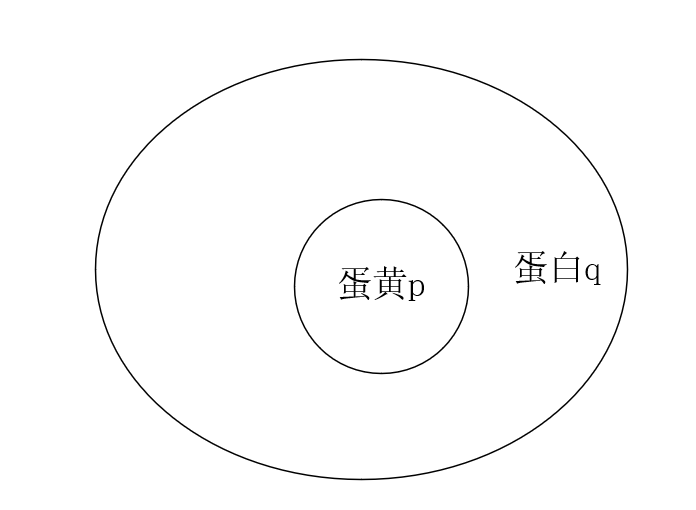
\includegraphics[width=0.5\textwidth]{Figure/若p则q.png}
            \caption{蕴含关系}
        \end{figure}

        p等价于q：$p \leftrightarrow q$，读作“p等价于q”，当p和q具有相同的真值时$p \leftrightarrow q$为真，否则为假。（数电的同或）。注意，真值等价则命题等价，与命题内容无关。

        \subsection{命题公式及分类}
            \subsubsection{命题公式的分类}
            \begin{enumerate}
            \item 命题公式不是命题，其真值是不确定的
            \item 合式公式：
                \begin{enumerate}
                    \item 由命题变元和联结词或括号进行一定连接的叫合式公式
                    \item 性质：
                        \begin{enumerate}
                            \item 若括号不影响运算次序的时候可以将括号省去
                            \item 合式公式和联结词组成的公式还是合式公式
                            \item 如果一个公式在各种赋值下都为真，则为\textbf{永真式}或\textbf{重言式}，反之\textbf{永假式}或\textbf{矛盾式}。至少有一个为真则称为\textbf{可满足式}
                        \end{enumerate}
                \end{enumerate}
            \end{enumerate}
            \subsubsection{构造真值表}

    \subsection{等值演算}
        如果两个命题公式的真值表完全相等，那么这俩就是等值式。

        若等价式$A\leftrightarrow B$是重言式，那么A和B称为等值式，记作$A\Leftrightarrow B$

        等值演算的性质如表\ref{等值演算的性质}所示：
        \renewcommand{\arraystretch}{1.5}
        \begin{table}[htbp]
            \centering
            \caption{等值演算的性质}\label{等值演算的性质}
            \small
            \begin{tabular}{ccc}
                \toprule
                序号 & 名称 & 等值式 \\
                \midrule
                1 & 双重否定律 & $A \Leftrightarrow \neg \neg A$ \\
                2 & 幂等律 & $A\Leftrightarrow A\vee A,\ A\Leftrightarrow A\wedge A$ \\
                3 & 交换律 & $A\vee B \Leftrightarrow B \vee A,\ A\wedge B \Leftrightarrow B \wedge A$ \\
                4 & 分配律 & $A\vee(B\wedge C)\Leftrightarrow (A\vee B)\wedge(A\vee C)$，记作$(A+B)*(A+C)$；\\
                  &         & $A\wedge(B\vee C)\Leftrightarrow (A \wedge B)\vee(A\wedge C)$，记作$A*(B+C)=AB+AC$ \\
                5 & 吸收律 & $A\vee (A\wedge B)\Leftrightarrow A,\ A\wedge(A\vee B)\Leftrightarrow A$ \\
                6 & 蕴含等值式 & $A\rightarrow B\Leftrightarrow \neg A\vee B$（箭头变或，前件加非）\\
                7 & 结合律 & $A\vee(B\vee C)\Leftrightarrow(A\vee B)\vee C,\ A\wedge(B\wedge C)\Leftrightarrow(A\wedge B)\wedge C$ \\
                8 & 德摩根律 & $\neg(A\vee B)\Leftrightarrow \neg A\wedge\neg B,\ \neg(A\wedge B)\Leftrightarrow \neg A\vee\neg B$ \\
                9 & 同一律 & $A\vee 0\Leftrightarrow A,\ A\wedge 1\Leftrightarrow A$ \\
                10 & 排中律 & $A\vee\neg A\Leftrightarrow 1$ \\
                11 & 矛盾律 & $A\wedge\neg A\Leftrightarrow 0$ \\
                12 & 等价等值式 & $A\leftrightarrow B\Leftrightarrow (A\rightarrow B)\wedge(B\rightarrow A)$ \\
                \bottomrule
            \end{tabular}
        \end{table}
    \subsection{范式}
        \begin{enumerate}
            \item 仅由\textbf{有限个命题变元}或其否定构成的析取式称为\textbf{简单析取式},同理有\textbf{简单合取式}
            \item 仅由\textbf{有限个简单合取式}构成的\textbf{析取式}称为\textbf{析取范式}如$(p\wedge q)\vee(p\wedge q)$，同理有，由有限个简单析取式构成的合取式称为\textbf{合取范式}
            \item 在$n$个命题变元中，若在\textbf{简单合取式}中的每个命题变元与其否定有且仅有一个\textbf{出现一次}则称这样的简单合取式为\textbf{极小项}，若全是最小项则称为\textbf{主析取范式}，同理有\textbf{极大项}，若全是极大项则称为\textbf{主合取范式}。
            \subsubsection{极小项是什么}
                对于含有 $n$ 个命题变元的命题公式，每一个极小项都是由这 $n$ 个命题变元或其否定构成的合取式。也就是说，在一个极小项中，每个命题变元都恰好出现一次，且只能以原命题或否定命题的形式出现。

                例如，对于两个命题变元 $p$ 和 $q$，其极小项共有 $2^2=4$ 个，分别为：
                \[
                \begin{aligned}
                m_0 &= \neg p \land \neg q,\\
                m_1 &= \neg p \land q,\\
                m_2 &= p \land \neg q,\\
                m_3 &= p \land q.
                \end{aligned}
                \]
                极小项的特点是：每一个极小项只在唯一一种真值赋值情况下为真，在其他赋值情况下均为假。例如：
                \[
                p \land \neg q
                \]
                只有在 $p$ 为真、$q$ 为假时为真。

                \subsubsection{极大项是什么}
                对于含有 $n$ 个命题变元的命题公式，每一个极大项都是由这 $n$ 个命题变元或其否定构成的析取式。也就是说，在一个极大项中，每个命题变元都恰好出现一次，且只能以原命题或否定命题的形式出现。

                例如，对于两个命题变元 $p$ 和 $q$，其极大项共有 $2^2=4$ 个，分别为：
                \[
                \begin{aligned}
                M_0 &= p \lor q,\\
                M_1 &= p \lor \neg q,\\
                M_2 &= \neg p \lor q,\\
                M_3 &= \neg p \lor \neg q.
                \end{aligned}
                \]

                极大项的特点是：每一个极大项只在唯一一种真值赋值情况下为假，在其他赋值情况下均为真。例如：
                \[
                p \lor \neg q
                \]
                只有在 $p$ 为假、$q$ 为真时为假。
            \item 任何命题公式都有唯一的主析取范式（但命题公式的析取范式和合取范式不唯一）
            \item 命题公式的类型
                \begin{enumerate}
                    \item 命题公式A为重言式：当且仅当A的主析取范式中\textbf{包含全部$2^n$个极小项}
                    \item 命题公式A为矛盾式：当且仅当A的主析取范式中\textbf{不包含任何极小项}
                    \item 命题公式A为可满足式：当且仅当A的主析取范式中\textbf{至少包含一个极小项}
                \end{enumerate}
        \end{enumerate}
    \newpage
\section{一阶逻辑}
    \subsection{一阶逻辑基本概念}
        \begin{enumerate}
            \item 个体常项：表示个体的名称，如a、b、c等。
            \item 个体变项：表示个体的变量，如x、y、z等。
            \item 谓词：表示个体之间的关系或属性，如P(x)、Q(x,y)等。
            \item 函数：表示个体之间的映射关系，如f(x)、g(x,y)等。
            \item 量词：表示个体的范围，如全称量词$\forall$和存在量词$\exists$。
            \item 元数：谓词或函数的参数个数，如P(x)是一个一元谓词，Q(x,y)是一个二元谓词。无参数的谓词或函数称为零元谓词或函数。
            \item 个体域：个体变项所取值的范围，如自然数、实数等。
        \end{enumerate}
        例题（将个体域默认为全人类）：
        \begin{enumerate}
            \item 所有人的人都要死，将其符号化为：
                \begin{equation}
                    \forall xF(x)
                \end{equation}
                其中，F(x)：x是要死的。这个命题是真命题
            \item 有的人活百岁以上，将其符号化为：
                \begin{equation}
                    \exists xG(x)
                \end{equation}
                其中，G(x)：x是活百岁以上的。这个命题是真命题
        \end{enumerate}

        若个体域D不为全人类，为全总个体域，即全宇宙的一切事物，则上述符号化不能成立。即$\forall xF(x)$表示的是全宇宙的一切事物都要死。而原命题意思是全人类都要死。不符合原命题的意思。

        因此引入一个新的谓词：特性谓词$M(x)$:x是人。则上述命题可以符号化为：
        \begin{equation}{\label{例题:所有人都要死}}
            \forall x(M(x)\rightarrow F(x))
        \end{equation}
        \begin{equation}{\label{例题:有的人活百岁以上}}
            \exists x(M(x)\wedge G(x))
        \end{equation}
        
        关于这部分什么时候用右箭头、什么时候用合取：
        \begin{enumerate}
            \item 所有满足 $M(x)$ 的东西，都满足 $F(x)$：
            \[
            \forall x(\text{范围} \rightarrow \text{性质})
            \]

            公式~\ref{例题:所有人都要死}表示的是：对于个体域中的任意一个对象 $x$，如果 $x$ 是人，即满足 $M(x)$，那么 $x$ 就要死，即满足 $F(x)$。因此这里用 $\rightarrow$ 表示由“是人”推出“要死”。

            \item 至少有一个东西，同时满足 $M(x)$ 和 $G(x)$：
            \[
            \exists x(\text{范围} \land \text{性质})
            \]

            公式~\ref{例题:有的人活百岁以上}表示的是：在个体域中至少存在一个对象 $x$，这个对象既是人，即满足 $M(x)$，又活百岁以上，即满足 $G(x)$。因此这里用 $\land$ 表示两个条件需要同时成立。同时满足是人（M(x)）和活百岁以上（G(x)）。如果使用 $\rightarrow$，则会表示为：存在一个对象 $x$，如果 $x$ 是人，那么 $x$ 就活百岁以上，这与原命题的意思不符。
        \end{enumerate}

        在使用量词时应注意以下情况
        \begin{enumerate}
            \item 如果事先没给出个体域，则默认为全总个体域。
            \item 个体域和谓词的含义确定后，$n$元谓词要转化为命题至少需要$n$个量词。
            \item 多个量词同时出现时不能随意颠倒顺序，颠倒后含义可能不同。
        \end{enumerate}
    \subsection{一阶逻辑合式公式及解释}
        字母表如表~\ref{tab:谓词逻辑基本符号}所示：
\begin{table}[htbp]
    \centering
    \caption{谓词逻辑中的基本符号}
    \label{tab:谓词逻辑基本符号}
    {\fontsize{10.5pt}{15pt}\selectfont
    \begin{tabular}{cll}
        \toprule
         符号类型 & 符号表示 \\
        \midrule
        个体常项 & $a,b,c,\dots$ \\
        个体变项 & $x,y,z,\dots$ \\
        函数符号 & $f,g,h,\dots$ \\
        谓词符号 & $P,Q,R,\dots$ \\
        逻辑联结词 & $\neg,\ \wedge,\ \vee,\ \rightarrow,\ \leftrightarrow$ \\
        量词 & $\forall$（全称量词）、$\exists$（存在量词） \\
        \bottomrule
    \end{tabular}
    }
\end{table}
    \subsection{原子公式与合式公式}
        \subsubsection{原子公式}
        原子公式就是没有被非$\neg$、合取$\wedge$、析取$\vee$、蕴含$\rightarrow$、任意$\forall$、存在$\exists$”等符号进一步组合的最基本公式。
        \subsubsection{合式公式}
        \begin{enumerate}
            \item 原子公式是合式公式（但合式公式不一定是原子公式）
            \item 若$A$是合式公式，则$\neg A$也是合式公式
            \item 若$A$、$B$是合式公式，则$A\wedge B$、$A \vee B$、$A\rightarrow B$、$A\leftrightarrow B$也是合式公式
            \item 若$A$是合式公式，则$\forall xA$、$\exists xA$也是合式公式
            \item 只有有限次的使用如上定义构成的符号串才是合式公式
        \end{enumerate}
        
        闭式：若公式$A$中无自由出现的个体变项，则称$A$是封闭的合式公式（比如$\forall xF(x)$是闭式，$\forall xF(x,y)$不是闭式，因为y没有被$\forall x$约束）
\end{document}